\chapter{Introduction}

\section{Motivation}

Amongst all robot types, humanoid robots are one of the most versatile robots when it comes to acting in a world with man-made structures and tools. As such, they are a huge area of research involving multiple disciplines. Of special research interest is humanoid manipulation using manipulators that resemble human hands. Manipulators with several degree of freedom (DoF) enable robots to reuse man-made tools for solving different kind of problems as opposed to be restricted to task-specific manipulators. Some of the tasks defined for the DARPA robotics challenge 2015 (DRC) \cite{DRC2013} intended to advance robotic manipulation into this direction by setting a robot in a rescue scenario that involves the interaction with door handles (Door task), turning valves (Valve task), connecting a hose to a wye (Hose task) and using a drill to cut a hole in a wall (Wall task). Since the DRC rules stated that the robot needed to carry all of its manipulators during each trial, teams were force to use versatile manipulators.

The advantage of having such a generic manipulator comes with the cost of more complex control. Humanoid manipulation does not only involve the grasping of a tool but also the continuous control of this tool for the duration of the task. Since grasped tools are only indirectly connected to the robot's kinematic chain, additional perceptual information is needed to estimate and track the actual state of the manipulated object.


\section{Problem Definition and Research Aim}

Humanoid manipulation is a challenging task because of two main reasons: inaccurate forward kinematics and changing environment.
Inaccurate forward kinematics is mostly caused by improper calibrated joint encoders and linkage elasticity. Both issues can only be resolved to some extent by e.g. modelling joint position offsets \cite{Fallon2015} and stiffness coefficients \cite{Johnson2015}. The effect of inaccurate forward kinematics is visualised in \cref{fig:calibration_issue}. Even small deviations in the reported joint positions propagate through the kinematic chain towards the manipulator and result in an offset that makes open-loop grasping infeasible.
By interacting with objects such as a valve, the robot needs to compensate the applied force by a whole body motion which likely changes the pose of the manipulated object in the camera frame.

\begin{figure}
\captionsetup{width=0.6\textwidth}
\centering
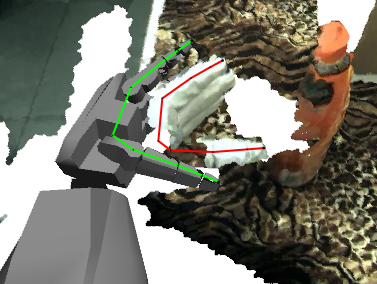
\includegraphics[width=0.5\textwidth]{images/valkyrie/joint_calibration_issue.png}
\caption[Joint calibration issue]{Joint calibration issue resulting in offset of reported pose (solid gray mesh, green marker) from perceived hand pose (coloured point cloud, red marker).}
\label{fig:calibration_issue}
\end{figure}

Both issues are in contrast with open-loop industrial robot applications such as moving parts in an assembly line, where stiff actuators manipulate objects at defined poses. Using visual feedback to estimate the configuration of the manipulator and the pose of the manipulated object could be the key step to enable closed-loop manipulation.
In return, visual tracking of highly articulated manipulators and objects causes interesting research questions itself again.

\paragraph{Manipulator tracking}
The main problem of tracking highly articulated manipulators with several degree of freedom is the large variety of their appearance. Using classical object detection methods on this problem would require an enormous amount of training data containing different configurations at different lighting conditions. In addition, classification results must be provided at real-time. On one side, the problem can be simplified in the context where a robot is observing its own manipulator by using a robot model representation and its joint encoder values. On the other side, the before mentioned issue of inaccurate forward kinematics reduces the utility of these encoder values.

As \emph{primary aim}, this thesis is investigating the effect of using visual perception and reported joint encoder values in conjunction to enable tracking when either of the two information is not available or inaccurate.

\paragraph{Object tracking}
In contrast to the manipulator, we usually have no prior information about the pose of the object up to the point where the manipulator gets in contact with the object. The Amazon Picking Challenge 2015 \cite{Correll2016} showed that detection and tracking of ordinary consumer products is still a challenging task. Amongst the 25 products used in the challenge were objects of varying appearance (e.g. non rigid objects), objects with meshed material (such as bins) and objects with reflective and translucent material. Classical machine learning approaches that rely on descriptive keypoint features such as SIFT fail in cases where textual information is not available either because of lighting conditions or material properties.

The \emph{secondary aim} of this thesis is the investigation of object tracking with lack of texture.


\section{Outline}

The current state of the art will be reviewed in \cref{sec:related_work} followed by a conclusion and a statement of the thereon based contribution of this work. The core properties of the DART algorithm, on which this work is based on, will be presented and discussed in \cref{sec:methods}, which also includes the extensions proposed in this work and the evaluation platform and methods. The extensions to the presented tracking approach will be evaluated in \cref{sec:evaluation} and compared to the base implementation. This work will conclude in \cref{sec:conclusion} with a summarized discussion of the results and propose future work for contributing to the research on articulated manipulator and object tracking.
